% Options for packages loaded elsewhere
\PassOptionsToPackage{unicode}{hyperref}
\PassOptionsToPackage{hyphens}{url}
\PassOptionsToPackage{dvipsnames,svgnames,x11names}{xcolor}
%
\documentclass[
  11pt,
]{article}

\usepackage{amsmath,amssymb}
\usepackage{setspace}
\usepackage{iftex}
\ifPDFTeX
  \usepackage[T1]{fontenc}
  \usepackage[utf8]{inputenc}
  \usepackage{textcomp} % provide euro and other symbols
\else % if luatex or xetex
  \usepackage{unicode-math}
  \defaultfontfeatures{Scale=MatchLowercase}
  \defaultfontfeatures[\rmfamily]{Ligatures=TeX,Scale=1}
\fi
\usepackage{lmodern}
\ifPDFTeX\else  
    % xetex/luatex font selection
    \setmainfont[]{Times New Roman}
\fi
% Use upquote if available, for straight quotes in verbatim environments
\IfFileExists{upquote.sty}{\usepackage{upquote}}{}
\IfFileExists{microtype.sty}{% use microtype if available
  \usepackage[]{microtype}
  \UseMicrotypeSet[protrusion]{basicmath} % disable protrusion for tt fonts
}{}
\makeatletter
\@ifundefined{KOMAClassName}{% if non-KOMA class
  \IfFileExists{parskip.sty}{%
    \usepackage{parskip}
  }{% else
    \setlength{\parindent}{0pt}
    \setlength{\parskip}{6pt plus 2pt minus 1pt}}
}{% if KOMA class
  \KOMAoptions{parskip=half}}
\makeatother
\usepackage{xcolor}
\usepackage[margin=1in]{geometry}
\setlength{\emergencystretch}{3em} % prevent overfull lines
\setcounter{secnumdepth}{5}
% Make \paragraph and \subparagraph free-standing
\makeatletter
\ifx\paragraph\undefined\else
  \let\oldparagraph\paragraph
  \renewcommand{\paragraph}{
    \@ifstar
      \xxxParagraphStar
      \xxxParagraphNoStar
  }
  \newcommand{\xxxParagraphStar}[1]{\oldparagraph*{#1}\mbox{}}
  \newcommand{\xxxParagraphNoStar}[1]{\oldparagraph{#1}\mbox{}}
\fi
\ifx\subparagraph\undefined\else
  \let\oldsubparagraph\subparagraph
  \renewcommand{\subparagraph}{
    \@ifstar
      \xxxSubParagraphStar
      \xxxSubParagraphNoStar
  }
  \newcommand{\xxxSubParagraphStar}[1]{\oldsubparagraph*{#1}\mbox{}}
  \newcommand{\xxxSubParagraphNoStar}[1]{\oldsubparagraph{#1}\mbox{}}
\fi
\makeatother


\providecommand{\tightlist}{%
  \setlength{\itemsep}{0pt}\setlength{\parskip}{0pt}}\usepackage{longtable,booktabs,array}
\usepackage{calc} % for calculating minipage widths
% Correct order of tables after \paragraph or \subparagraph
\usepackage{etoolbox}
\makeatletter
\patchcmd\longtable{\par}{\if@noskipsec\mbox{}\fi\par}{}{}
\makeatother
% Allow footnotes in longtable head/foot
\IfFileExists{footnotehyper.sty}{\usepackage{footnotehyper}}{\usepackage{footnote}}
\makesavenoteenv{longtable}
\usepackage{graphicx}
\makeatletter
\def\maxwidth{\ifdim\Gin@nat@width>\linewidth\linewidth\else\Gin@nat@width\fi}
\def\maxheight{\ifdim\Gin@nat@height>\textheight\textheight\else\Gin@nat@height\fi}
\makeatother
% Scale images if necessary, so that they will not overflow the page
% margins by default, and it is still possible to overwrite the defaults
% using explicit options in \includegraphics[width, height, ...]{}
\setkeys{Gin}{width=\maxwidth,height=\maxheight,keepaspectratio}
% Set default figure placement to htbp
\makeatletter
\def\fps@figure{htbp}
\makeatother
% definitions for citeproc citations
\NewDocumentCommand\citeproctext{}{}
\NewDocumentCommand\citeproc{mm}{%
  \begingroup\def\citeproctext{#2}\cite{#1}\endgroup}
\makeatletter
 % allow citations to break across lines
 \let\@cite@ofmt\@firstofone
 % avoid brackets around text for \cite:
 \def\@biblabel#1{}
 \def\@cite#1#2{{#1\if@tempswa , #2\fi}}
\makeatother
\newlength{\cslhangindent}
\setlength{\cslhangindent}{1.5em}
\newlength{\csllabelwidth}
\setlength{\csllabelwidth}{3em}
\newenvironment{CSLReferences}[2] % #1 hanging-indent, #2 entry-spacing
 {\begin{list}{}{%
  \setlength{\itemindent}{0pt}
  \setlength{\leftmargin}{0pt}
  \setlength{\parsep}{0pt}
  % turn on hanging indent if param 1 is 1
  \ifodd #1
   \setlength{\leftmargin}{\cslhangindent}
   \setlength{\itemindent}{-1\cslhangindent}
  \fi
  % set entry spacing
  \setlength{\itemsep}{#2\baselineskip}}}
 {\end{list}}
\usepackage{calc}
\newcommand{\CSLBlock}[1]{\hfill\break\parbox[t]{\linewidth}{\strut\ignorespaces#1\strut}}
\newcommand{\CSLLeftMargin}[1]{\parbox[t]{\csllabelwidth}{\strut#1\strut}}
\newcommand{\CSLRightInline}[1]{\parbox[t]{\linewidth - \csllabelwidth}{\strut#1\strut}}
\newcommand{\CSLIndent}[1]{\hspace{\cslhangindent}#1}

\usepackage{xcolor}
\definecolor{navyblue}{RGB}{0, 0, 128}
\definecolor{lightblue}{RGB}{102, 178, 255}

% Title formatting: navy blue, centered, large font
\usepackage{titling}
\pretitle{\begin{center}\Huge\color{navyblue}\bfseries}
\posttitle{\par\end{center}\vskip 0.5em}

% Section and subsection headers color
\usepackage{sectsty}
\sectionfont{\color{lightblue}}      % Sections in light blue
\subsectionfont{\color{lightblue}}   % Subsections in light blue

\makeatletter
\@ifpackageloaded{caption}{}{\usepackage{caption}}
\AtBeginDocument{%
\ifdefined\contentsname
  \renewcommand*\contentsname{Table of contents}
\else
  \newcommand\contentsname{Table of contents}
\fi
\ifdefined\listfigurename
  \renewcommand*\listfigurename{List of Figures}
\else
  \newcommand\listfigurename{List of Figures}
\fi
\ifdefined\listtablename
  \renewcommand*\listtablename{List of Tables}
\else
  \newcommand\listtablename{List of Tables}
\fi
\ifdefined\figurename
  \renewcommand*\figurename{Figure}
\else
  \newcommand\figurename{Figure}
\fi
\ifdefined\tablename
  \renewcommand*\tablename{Table}
\else
  \newcommand\tablename{Table}
\fi
}
\@ifpackageloaded{float}{}{\usepackage{float}}
\floatstyle{ruled}
\@ifundefined{c@chapter}{\newfloat{codelisting}{h}{lop}}{\newfloat{codelisting}{h}{lop}[chapter]}
\floatname{codelisting}{Listing}
\newcommand*\listoflistings{\listof{codelisting}{List of Listings}}
\makeatother
\makeatletter
\makeatother
\makeatletter
\@ifpackageloaded{caption}{}{\usepackage{caption}}
\@ifpackageloaded{subcaption}{}{\usepackage{subcaption}}
\makeatother

\ifLuaTeX
  \usepackage{selnolig}  % disable illegal ligatures
\fi
\usepackage{bookmark}

\IfFileExists{xurl.sty}{\usepackage{xurl}}{} % add URL line breaks if available
\urlstyle{same} % disable monospaced font for URLs
\hypersetup{
  pdftitle={COVID-19 Impact Analysis: Cases, Deaths, and Vaccination Rates Across Six Countries},
  pdfauthor={Lin Qi, Midhun Unnikrishnan, and Sumintra Boonmat},
  colorlinks=true,
  linkcolor={blue},
  filecolor={Maroon},
  citecolor={Blue},
  urlcolor={blue},
  pdfcreator={LaTeX via pandoc}}


\title{COVID-19 Impact Analysis: Cases, Deaths, and Vaccination Rates
Across Six Countries}
\author{Lin Qi, Midhun Unnikrishnan, and Sumintra Boonmat}
\date{}

\begin{document}
\maketitle

\renewcommand*\contentsname{Table of contents}
{
\hypersetup{linkcolor=}
\setcounter{tocdepth}{3}
\tableofcontents
}

\setstretch{1.5}
\section{Executive Summary}\label{sec-intro}

This report details a study of COVID-19 confirmed cases, deaths, and
vaccination rates across Canada, France, Germany, India, the UK, and the
US from February 2020 to July 2023. It shows the impact of vaccination
on pandemic outcomes. Studies state that countries, including the US and
UK, saw a decrease in both cases and deaths when vaccination uptake
began at the onset of the pandemic. This analysis shows how vaccination
has a proportionately large effect relative to decreasing pandemic
numbers.

\section{Introduction}\label{introduction}

Since early 2020, countries around the globe have experienced COVID-19
to different extents. Governments responded with measures like testing,
lockdowns, and mass vaccination, but the outcomes varied significantly.
This study compares Canada, France, Germany, India, the UK, and the US
to understand the contrast in outcomes. It researches time series data
on confirmed cases, deaths, and vaccination rates from 2020 to 2023. The
primary question focuses on the role of vaccination in decreasing case
numbers and mortality rates. Vaccination programs started at varying
times, with richer nations beginning earlier. For example, Canada and
the United States started vaccinations in December 2020, while India
began in January 2021. This study aims to provide insight into
successful responses to the pandemic. It highlights the importance of
vaccination in reducing the spread and severity of the virus.

\section{Methodology}\label{sec-method}

\textbf{Data Source}:

We used publicly available datasets from Our World in Data, including:

\begin{itemize}
\item
  Confirmed COVID-19 case numbers (Ritchie et al. 2020a)
\item
  COVID-19 death data (Ritchie et al. 2020b)
\item
  COVID-19 vaccination data (Ritchie et al. 2020c)
\end{itemize}

\textbf{Time Range Validation}:

\begin{itemize}
\item
  Confirmed Cases: February 1, 2020 - February 1, 2023
\item
  Death Rates: February 1, 2020 - February 1, 2023
\item
  Vaccination Data::
\end{itemize}

The vaccination dataset was obtained from Our World in Data. We observed
that different countries had different vaccination start and end dates.
For example, Canada and the US began recording vaccinations in December
2020, while India started in mid-January 2021. These differences are
likely due to unequal access to vaccines and different national data
reporting schedules.

To ensure fair comparisons, we limited our analysis to the overlapping
period across all six countries: from January 16, 2021 to September 4,
2022. This allows for consistent visualization and avoids bias caused by
missing early or late-stage data in certain countries.

\textbf{Data Cleaning and Preprocessing}:

Data cleaning was performed in R using the tidyverse and lubridate
packages. First, records with missing vaccination rates (doses per
million) were excluded using filter(!is.na(\ldots)) to keep consistency
in the analysis. Column names were standardized, and all datasets were
reshaped from wide to long format via pivot\_longer() to facilitate
merging.

Dates were parsed using ymd() to create uniform date objects. Death
data, initially provided per 100,000 people, was converted to per
million by multiplying by 10 to align with the scale of other variables.

The confirmed case and vaccination datasets were merged by country and
date. This combined data was further joined with the cleaned death
dataset to form a unified, time-aligned dataset with complete metrics
for each country.

\textbf{Data Analysis Strategy}:

The resulting dataset was used to explore trends in vaccination coverage
and pandemic progression through visualizations and a 7-day lag
analysis. Figure~\ref{fig-vacc-trend} illustrates the 7-day average
vaccination rate per million, highlighting varied rollout speeds.
Table~\ref{tbl-vacc-summary} summarizes the vaccination data coverage
period for each country, confirming early rollout in high-income
countries and delayed coverage in others.

These preprocessing steps ensured data quality, consistency, and
meaningful cross-country comparisons throughout the analysis.

\begin{figure}

\centering{

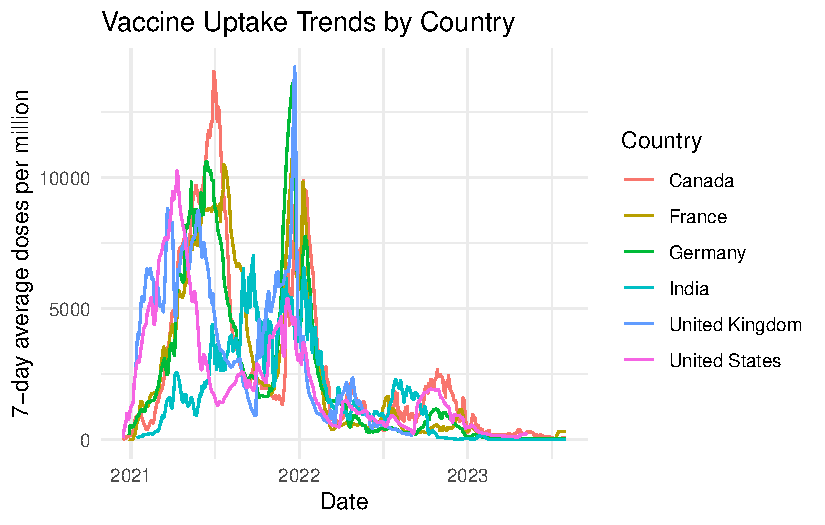
\includegraphics{Analysis_files/figure-pdf/fig-vacc-trend-1.pdf}

}

\caption{\label{fig-vacc-trend}Figure: COVID-19 vaccine: 7-day average
doses per million (by country)}

\end{figure}%

\begin{longtable}[]{@{}lll@{}}

\caption{\label{tbl-vacc-summary}Table: Summary of vaccination data
coverage (start-end date by country)}

\tabularnewline

\toprule\noalign{}
Country & Start & End \\
\midrule\noalign{}
\endhead
\bottomrule\noalign{}
\endlastfoot
Canada & 2020-12-15 & 2023-07-31 \\
France & 2020-12-28 & 2023-07-31 \\
Germany & 2020-12-28 & 2023-07-31 \\
India & 2021-01-16 & 2023-07-31 \\
United Kingdom & 2021-01-11 & 2022-09-04 \\
United States & 2020-12-15 & 2023-05-09 \\

\end{longtable}

\section{Results}\label{sec-results}

The analysis across six countries shows key patterns in the relationship
between COVID-19 cases, deaths, and vaccination.

The daily changes in COVID-19 case and vaccination rates in
Figure~\ref{fig-daily-change} shows that large outbreaks triggered
spikes in vaccination, indicating reactive public health responses.
Similarly, Figure~\ref{fig-vacc-vs-case}, shows that vaccines were often
given after case numbers had already started rising.

\begin{figure}

\centering{

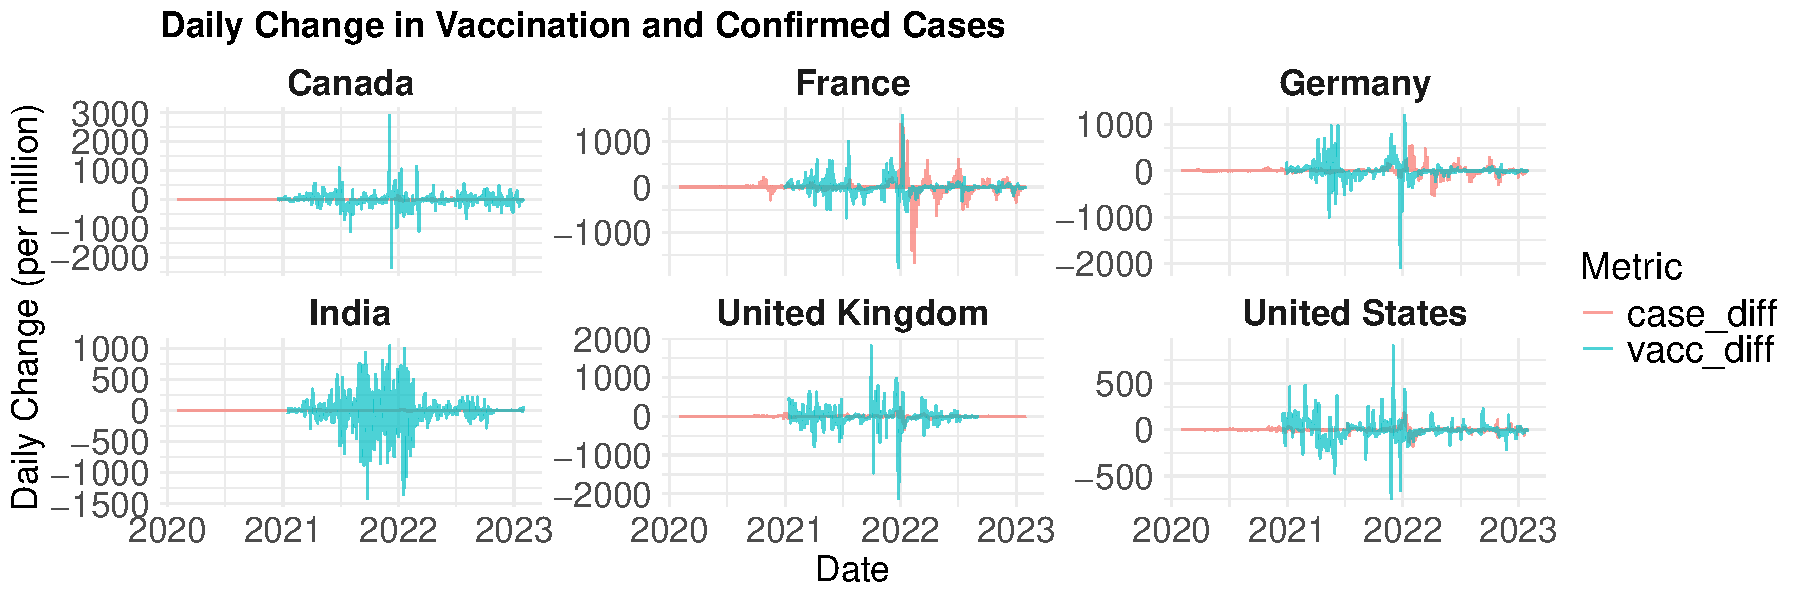
\includegraphics{Analysis_files/figure-pdf/fig-daily-change-1.pdf}

}

\caption{\label{fig-daily-change}Figure: Daily changes in confirmed
cases and vaccine doses per million}

\end{figure}%

\begin{figure}

\centering{

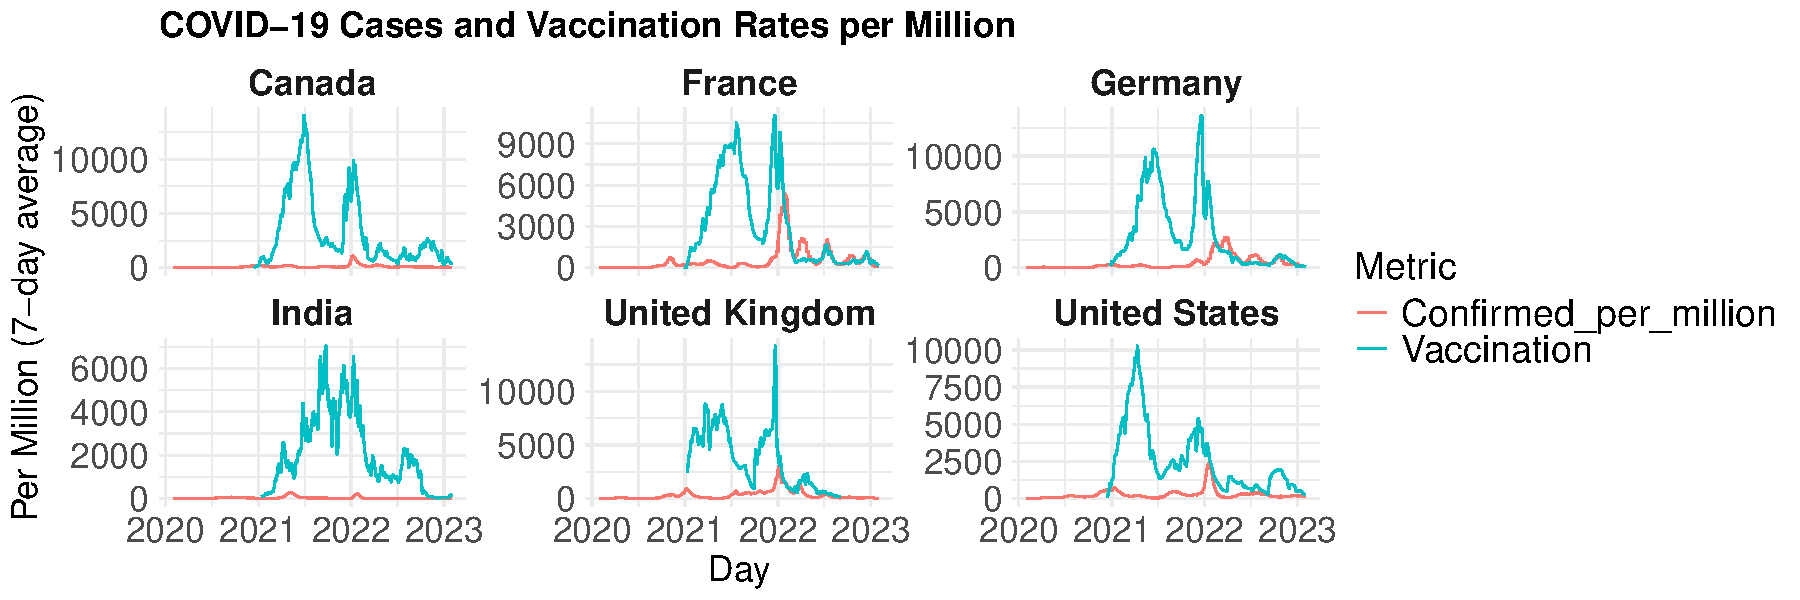
\includegraphics{Analysis_files/figure-pdf/fig-vacc-vs-case-1.pdf}

}

\caption{\label{fig-vacc-vs-case}Figure: Comparison of confirmed cases
and vaccination rates per million (by country)}

\end{figure}%

A 7-day lag analysis Figure~\ref{fig-lag-effect} shows that higher
vaccination rates were followed by declines in new case numbers,
particularly in countries like the US and UK. This suggests that
vaccines helped slow the spread of the virus.

\begin{figure}

\centering{

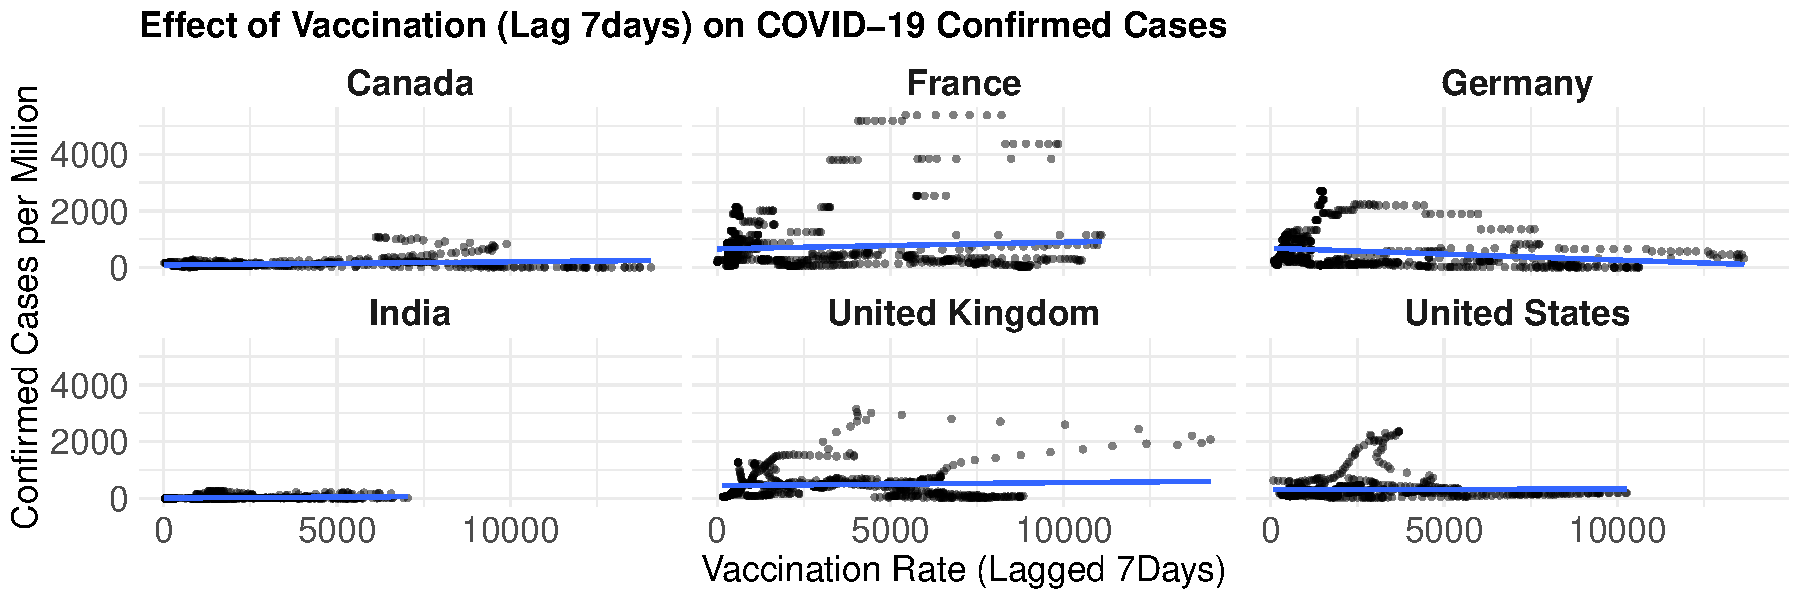
\includegraphics{Analysis_files/figure-pdf/fig-lag-effect-1.pdf}

}

\caption{\label{fig-lag-effect}Figure: Lagged vaccination rate vs
confirmed cases (7-day lag, by country)}

\end{figure}%

Figure~\ref{fig-case-death-vacc} illustrates the trends in confirmed
COVID-19 cases, deaths, and vaccination rates per million across six
countries. In the early stages of the pandemic, when vaccines were not
yet available, the number of deaths closely followed confirmed cases.
However, in later waves, as vaccination coverage expanded, deaths did
not rise in proportion to case numbers. This growing gap suggests that
vaccines played a key role in reducing the severity of outcomes, even
when transmission rates remained high.

The overall findings show that vaccination contributed to lower death
rates and reduced the impact of major outbreaks when implemented early
and consistently.

\begin{figure}

\centering{

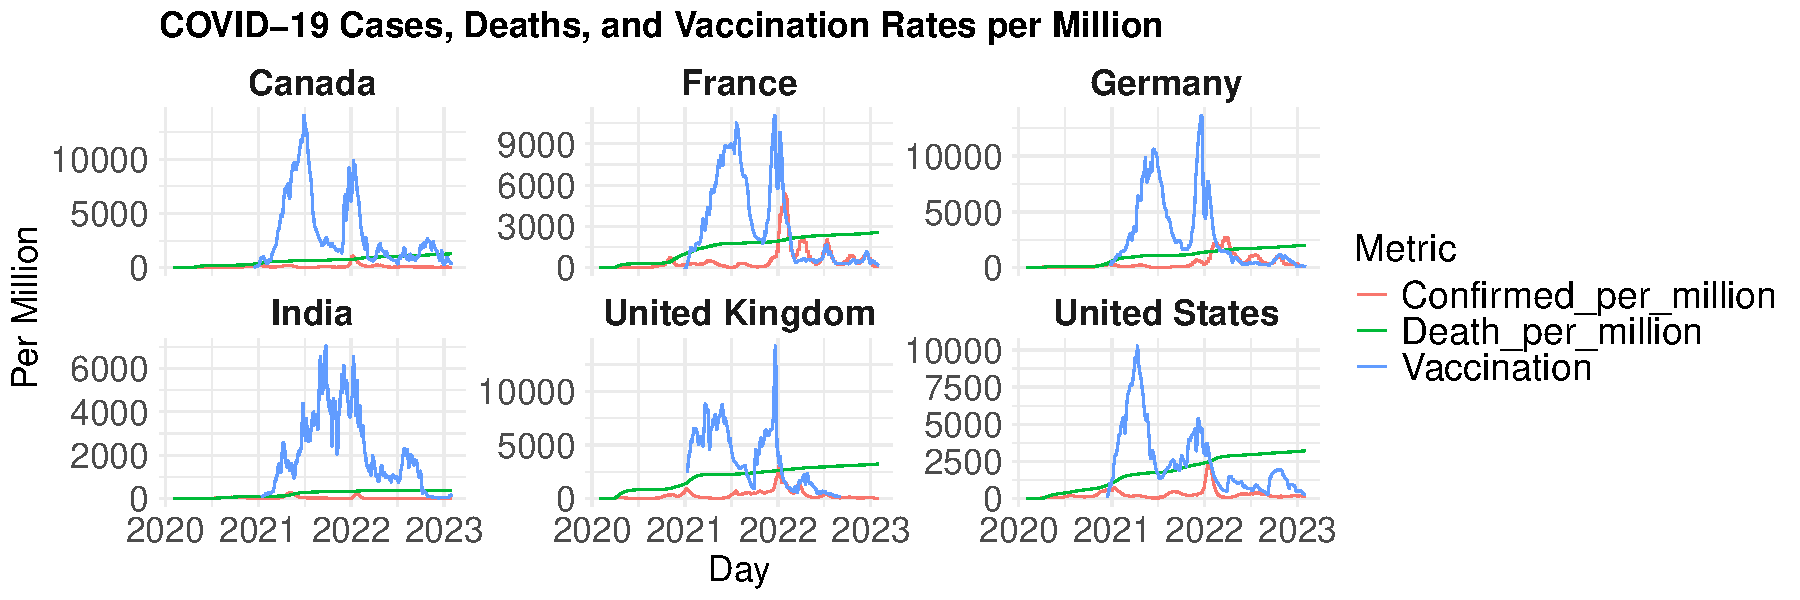
\includegraphics{Analysis_files/figure-pdf/fig-case-death-vacc-1.pdf}

}

\caption{\label{fig-case-death-vacc}Figure: COVID-19 confirmed
case-death rates-vaccination by country)}

\end{figure}%

\section{Discussion}\label{sec-discussion}

\begin{enumerate}
\def\labelenumi{\arabic{enumi}.}
\item
  Case rates depend heavily on how much testing was available and how
  consistently it was used. Some countries, particularly in early stages
  of the pandemic, had limited testing capacity, meaning many infections
  may have gone unrecorded. In contrast, countries with widespread and
  frequent testing likely reported more cases, even among people with
  mild or no symptoms.
\item
  The differences in how countries report COVID-19 deaths may affect the
  accuracy of comparisons. For example, some countries may only record
  deaths that occur in hospitals, while others include deaths that
  happen at home. This means that countries with more limited reporting
  systems could appear to have lower death rates, even if the actual
  impact was higher.
\end{enumerate}

\section{Conclusion}\label{sec-conclusion}

During the project, we analyzed numbers of confirmed cases, deaths and
vaccinations in Canada, France, Germany, India, the UK and the US.

Our findings highlight three key observations:

\begin{enumerate}
\def\labelenumi{\arabic{enumi}.}
\item
  In most countries, the number of cases increased quite a bit before
  widespread vaccination took place.
\item
  During major outbreaks, both case numbers and vaccine doses
  administered showed significant daily fluctuations.
\item
  A 7-day lag analysis indicated that rising vaccination rates were
  followed by a reduction in new case numbers. Areas where vaccination
  started early and was kept up showed the strongest impact.
\end{enumerate}

These insights suggest that timely and sustained vaccination campaigns
played a crucial role in reducing transmission and saving lives. Future
public health responses should prioritize early vaccine deployment
during pandemics.

\section{Recommendations}\label{sec-recommendations}

Given the findings, we suggest that further pandemic responses
concentrate on spreading vaccinations quickly, especially in
lower-income parts of the world like India, in order to reduce chances
for breaks in case numbers. As seen in Figure~\ref{fig-daily-change},
rather than waiting for a surge, Governments should consider
establishing proactive vaccination schemes, ensuring vaccines are
deployed before a high number of cases occur. Having comparable ways of
reporting data in different nations allows for better assessment and
guides effective policy creation. Finally such campaigns need to make
sure vaccination efforts continue, because sustained work in the US and
UK greatly reduced the number of people affected and the death rate, as
shown in Figure~\ref{fig-case-death-vacc}.

\section{References}\label{sec-references}

\phantomsection\label{refs}
\begin{CSLReferences}{1}{0}
\bibitem[\citeproctext]{ref-owid_covid_cases_2020}
Ritchie, Hannah, Edouard Mathieu, Lucas Rodés-Guirao, Cameron Appel,
Charlie Giattino, Esteban Ortiz-Ospina, Joe Hasell, Bobbie Macdonald,
Diana Beltekian, and Max Roser. 2020a. {``COVID-19 Confirmed Cases.''}
\url{https://ourworldindata.org/covid-cases}; Our World in Data.

\bibitem[\citeproctext]{ref-owid_covid_deaths_2020}
---------. 2020b. {``COVID-19 Deaths.''}
\url{https://ourworldindata.org/covid-deaths}; Our World in Data.

\bibitem[\citeproctext]{ref-owid_covid_vaccinations_2020}
---------. 2020c. {``COVID-19 Vaccinations.''}
\url{https://ourworldindata.org/covid-vaccinations}; Our World in Data.

\end{CSLReferences}




\end{document}
